\chapter{The Lamb Opens the Scroll (6:1--7:17)}

In heaven, the Lamb opens the seals; on earth, judgment unfolds.

The first four seals reveal judgment upon the earth through conquest, war, famine, and death. The fifth turns our gaze toward the souls of those who were martyred because of the word of God and their faithful testimony. When the sixth seal is opened, the heavens and the earth are shaken, and the stars fall from the sky. The great day of the Lamb's wrath has come, and the people of the earth cry out in terror: ``Who can withstand it?''

Revelation 7 answers this question. Only those who belong to God, cleansed by the blood of the Lamb, can stand before the throne and before the Lamb. Thus, the seven seals reveal not only the fearsome reality of divine judgment but also God's preserving care for His people, the salvation accomplished by the Lamb, and the eternal hope that awaits the redeemed.

\section{The First Four Seals: The Four Horsemen}

% Insert the licensed NIV text of Revelation 6:1--8 in the ScriptureBox below.

\begin{ScriptureBox}

\item[6:1] I watched as the Lamb opened the first of the seven seals. Then I heard one of the four living creatures say in a voice like thunder, ``Come!''

\item[6:2] I looked, and there before me was a white horse! Its rider held a bow, and he was given a crown, and he rode out as a conqueror bent on conquest.

\item[6:3] When the Lamb opened the second seal, I heard the second living creature say, ``Come!''

\item[6:4] Then another horse came out, a fiery red one. Its rider was given power to take peace from the earth and to make people kill each other. To him was given a large sword.

\item[6:5] When the Lamb opened the third seal, I heard the third living creature say, ``Come!'' I looked, and there before me was a black horse! Its rider was holding a pair of scales in his hand.

\item[6:6] Then I heard what sounded like a voice among the four living creatures, saying, ``Two pounds of wheat for a day's wages, and six pounds of barley for a day's wages, and do not damage the oil and the wine!''

\item[6:7] When the Lamb opened the fourth seal, I heard the voice of the fourth living creature say, ``Come!''

\item[6:8] I looked, and there before me was a pale horse! Its rider was named Death, and Hades was following close behind him. They were given power over a fourth of the earth to kill by sword, famine and plague, and by the wild beasts of the earth.

\end{ScriptureBox}

\begin{figure}[htbp]
    \centering
    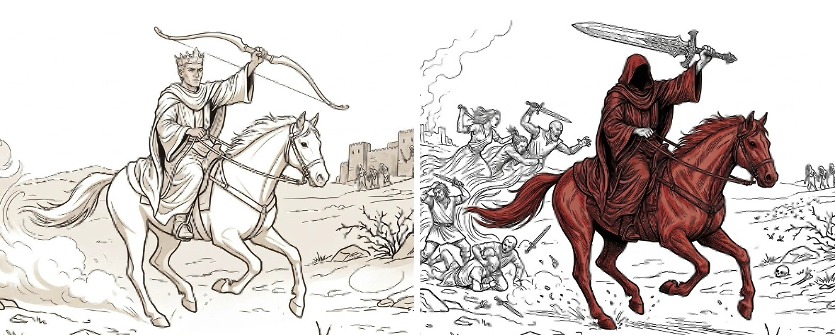
\includegraphics[
    width=1\textwidth,
    trim=0 0 0 00,
    clip]{images/horses_white_red.png}
    \caption{The 1st and 2nd Seals}
    \label{fig:horses_white_red.png}
\end{figure}

The four horses and their riders bring a succession of conquest, war, famine, and death upon the earth.

The white horse rides forth to conquer and conquer again. The red horse brings bloodshed. The black horse brings famine and poverty. The pale horse brings death.

I use the following mnemonic to help remember the distinctive role of each horse:

\begin{center}
\begin{tabular}{l}
\hline
White to conquer \\
Red to kill \\
Black to famine \\
Pale to die \\
\hline
\end{tabular}
\end{center}

\begin{figure}[htbp]
    \centering
    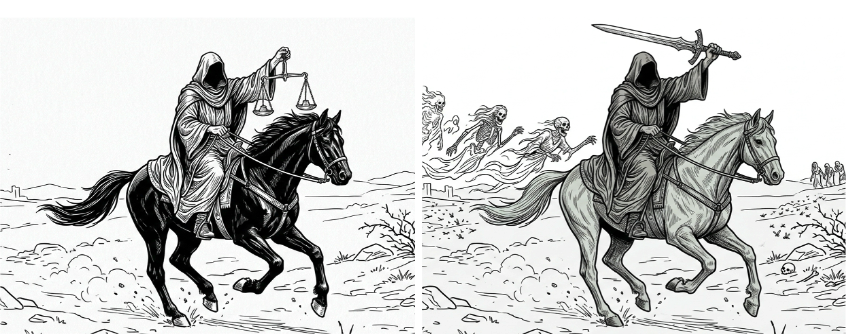
\includegraphics[
    width=1\textwidth,
    trim=0 0 0 0,
    clip]{images/horses_black_gray.png}
    \caption{The 3rd and 4th Seals}
    \label{fig:horses_black_gray.png}
\end{figure}

The words ``a quart of wheat for a day's wages'' portray the famine that often follows war, when food becomes scarce and prices soar. During wartime, armies frequently obtain provisions by plundering the countryside, sometimes seizing food by force and leaving villages stripped of their supplies. Famine is one of the devastating consequences that war leaves in its wake.

Wheat and barley were important staples throughout the Roman Empire. Wheat was generally considered the better grain and served as a principal food, while barley was less expensive and more commonly consumed by poorer people. A quart of wheat represented approximately one person's daily portion, while three quarts of barley provided a roughly comparable daily supply of grain.

A denarius, or silver coin, commonly represented a laborer's wages for one day's work. A person might therefore labor throughout the day only to earn enough to purchase the wheat needed for that day's food. Even if he bought barley instead, his wages would barely cover his basic portion. Supporting a family, paying for shelter, and meeting other daily expenses would be harder still.

This is the terrible condition the vision portrays: food remains available, but its price has risen beyond what ordinary people can reasonably afford. Olive oil and wine, even more precious in a time of scarcity, are not to be wasted. When even the daily necessities of life become difficult to obtain, every remaining resource matters.

The red, black, and pale horses are relatively straightforward to understand from the text. But who is the rider on the white horse? Biblical interpreters have generally proposed three major interpretations.

\begin{enumerate}

\item \textbf{The white horse represents a false Christ or the forces of the Antichrist.}

This is the view widely held by many futurist interpreters; see the appendix, ``Various Views of the End Times.''\footnote{MacArthur, J. (2007).}

The rider carries a bow, yet no arrows are mentioned. Some interpreters take this detail to suggest conquest through deception, political maneuvering, or the appearance of peaceful success. They also connect the rider with the beast and the forces of the Antichrist described later in Revelation. Thus, the first seal marks the beginning of the Antichrist's activity in the last days.

Matthew 24:4--5 warns that false messiahs will deceive many before Jesus speaks of wars and famines. The resemblance between the sequence in Matthew and the four horsemen lends support to this interpretation.

\item \textbf{The white horse represents military conquest.}

Other interpreters argue that the rider need not be the Antichrist. Since the text explicitly says that he went out ``as a conqueror bent on conquest,'' they understand him to symbolize military expansion and imperial aggression more generally.

Conquest often leads to war, famine, and death. Thus, the four horsemen form a connected sequence: the ambitions of conquest give rise to bloodshed, scarcity, and widespread mortality.

\item \textbf{The white horse represents Christ or the victory of the gospel.}

This is a less widely held interpretation. Those who support it point out that white often symbolizes holiness and victory in Revelation. In Revelation 19:11, Christ Himself rides a white horse, and the rider's continuing conquest in Revelation 6:2 may be understood as the advancing triumph of the gospel.

However, many modern interpreters do not accept this view. They argue that the four horsemen should be understood together as a unified group, and that significant differences remain between the rider in Revelation 6 and Christ on the white horse in Revelation 19.

\end{enumerate}

\section{The Fifth Seal: The Cry of the Martyrs}

% Insert the licensed NIV text of Revelation 6:9--11 in the ScriptureBox below.

\begin{ScriptureBox}

\item[6:9] When he opened the fifth seal, I saw under the altar the souls of those who had been slain because of the word of God and the testimony they had maintained.

\item[6:10] They called out in a loud voice, ``How long, Sovereign Lord, holy and true, until you judge the inhabitants of the earth and avenge our blood?''

\item[6:11] Then each of them was given a white robe, and they were told to wait a little longer, until the full number of their fellow servants, their brothers and sisters, were killed just as they had been.

\end{ScriptureBox}

In the eyes of many Romans, the followers of Jesus were misguided and superstitious. To give one's life in allegiance to a Messiah who had been crucified seemed absurd, even ridiculous. Some surviving historical records offer a sobering glimpse of the hostility Christians faced.\footnote{Koester, C. R. (2014).}\footnote{Tacitus, \textit{Ann.} 15.44; Pliny the Younger, \textit{Ep.} 10.96.8.}\footnote{\textit{Mart. Carp.} 9.}

The martyrs were killed because of the word of God and their testimony. They had remained faithful in proclaiming God's truth and bearing witness to Him, yet their faithfulness brought them suffering and death. What a profound injustice!

For Christians who faced persecution and martyrdom in the first century, this vision would have offered extraordinary comfort. Though rejected and killed on earth, the martyrs beneath the altar were not forgotten. They were received into God's presence, and their cries reached the ears of the Holy and True One.

Their testimony teaches us three important lessons:

\begin{enumerate}
\item Remain faithful in bearing witness to God, even when faithfulness demands the ultimate sacrifice (6:9).
\item Bring our grievances before the Holy and Righteous Lord rather than taking vengeance into our own hands (6:10).
\item While the fullness of justice is still awaited, receive God's assurance and continue to endure in faith (6:11).
\end{enumerate}

You may ask, however: Did the Lord Jesus not teach us to love our enemies and pray for those who persecute us? How, then, should we understand the martyrs' cry for justice?

The key is to recognize the injustice suffered by the victims. These believers were persecuted and killed because they remained loyal to Christ. Their appeal to God was not a demand for permission to take personal revenge. Rather, they entrusted judgment to the righteous Judge.

The passage assures us that the God who is holy and true does not forget those who faithfully follow Him and bear witness to His name. If the martyrs confess that God is ``holy and true,'' can He remain forever indifferent when the wicked shed innocent blood?

God's judgment comes at the time He has appointed. Even the completion of the number of martyrs belongs to His sovereign purpose. The final judgment will not occur according to human impatience, but according to God's perfect wisdom.

The fact that God does not immediately execute final judgment does not mean that He overlooks evil or has forgotten His promises. Rather, in His mercy and patience, He continues to give people an opportunity to repent. As 2 Peter 3:9--10 explains, the apparent delay of the Lord's promise reflects His patience and His desire that people should come to repentance. Yet the day of the Lord will come like a thief, and the present order will not endure forever.

The same patience that grants sinners time to turn back to God also calls His people to persevere. We may grieve over injustice, and we may cry out for the Lord to act. But we do so in the confidence that history remains in His hands and that His justice will not fail.

\section{The Sixth Seal: The Stars Fall from the Sky}

\begin{ScriptureBox}

\item[6:12] I watched as he opened the sixth seal. There was a great earthquake. The sun turned black like sackcloth made of goat hair, the whole moon turned blood red,

\item[6:13] and the stars in the sky fell to earth, as figs drop from a fig tree when shaken by a strong wind.

\item[6:14] The heavens receded like a scroll being rolled up, and every mountain and island was removed from its place.

\item[6:15] Then the kings of the earth, the princes, the generals, the rich, the mighty, and everyone else, both slave and free, hid in caves and among the rocks of the mountains.

\item[6:16] They called to the mountains and the rocks, ``Fall on us and hide us from the face of him who sits on the throne and from the wrath of the Lamb!

\item[6:17] For the great day of their wrath has come, and who can withstand it?''
% NIV footnotes for 6:16--17 (omitted; add as \footnote if wanted):
%   6:16 ``hide us'' --- See Hosea 10:8.
%   6:17 ``their'' --- Some manuscripts his
\end{ScriptureBox}

\begin{figure}[htbp]
    \centering
    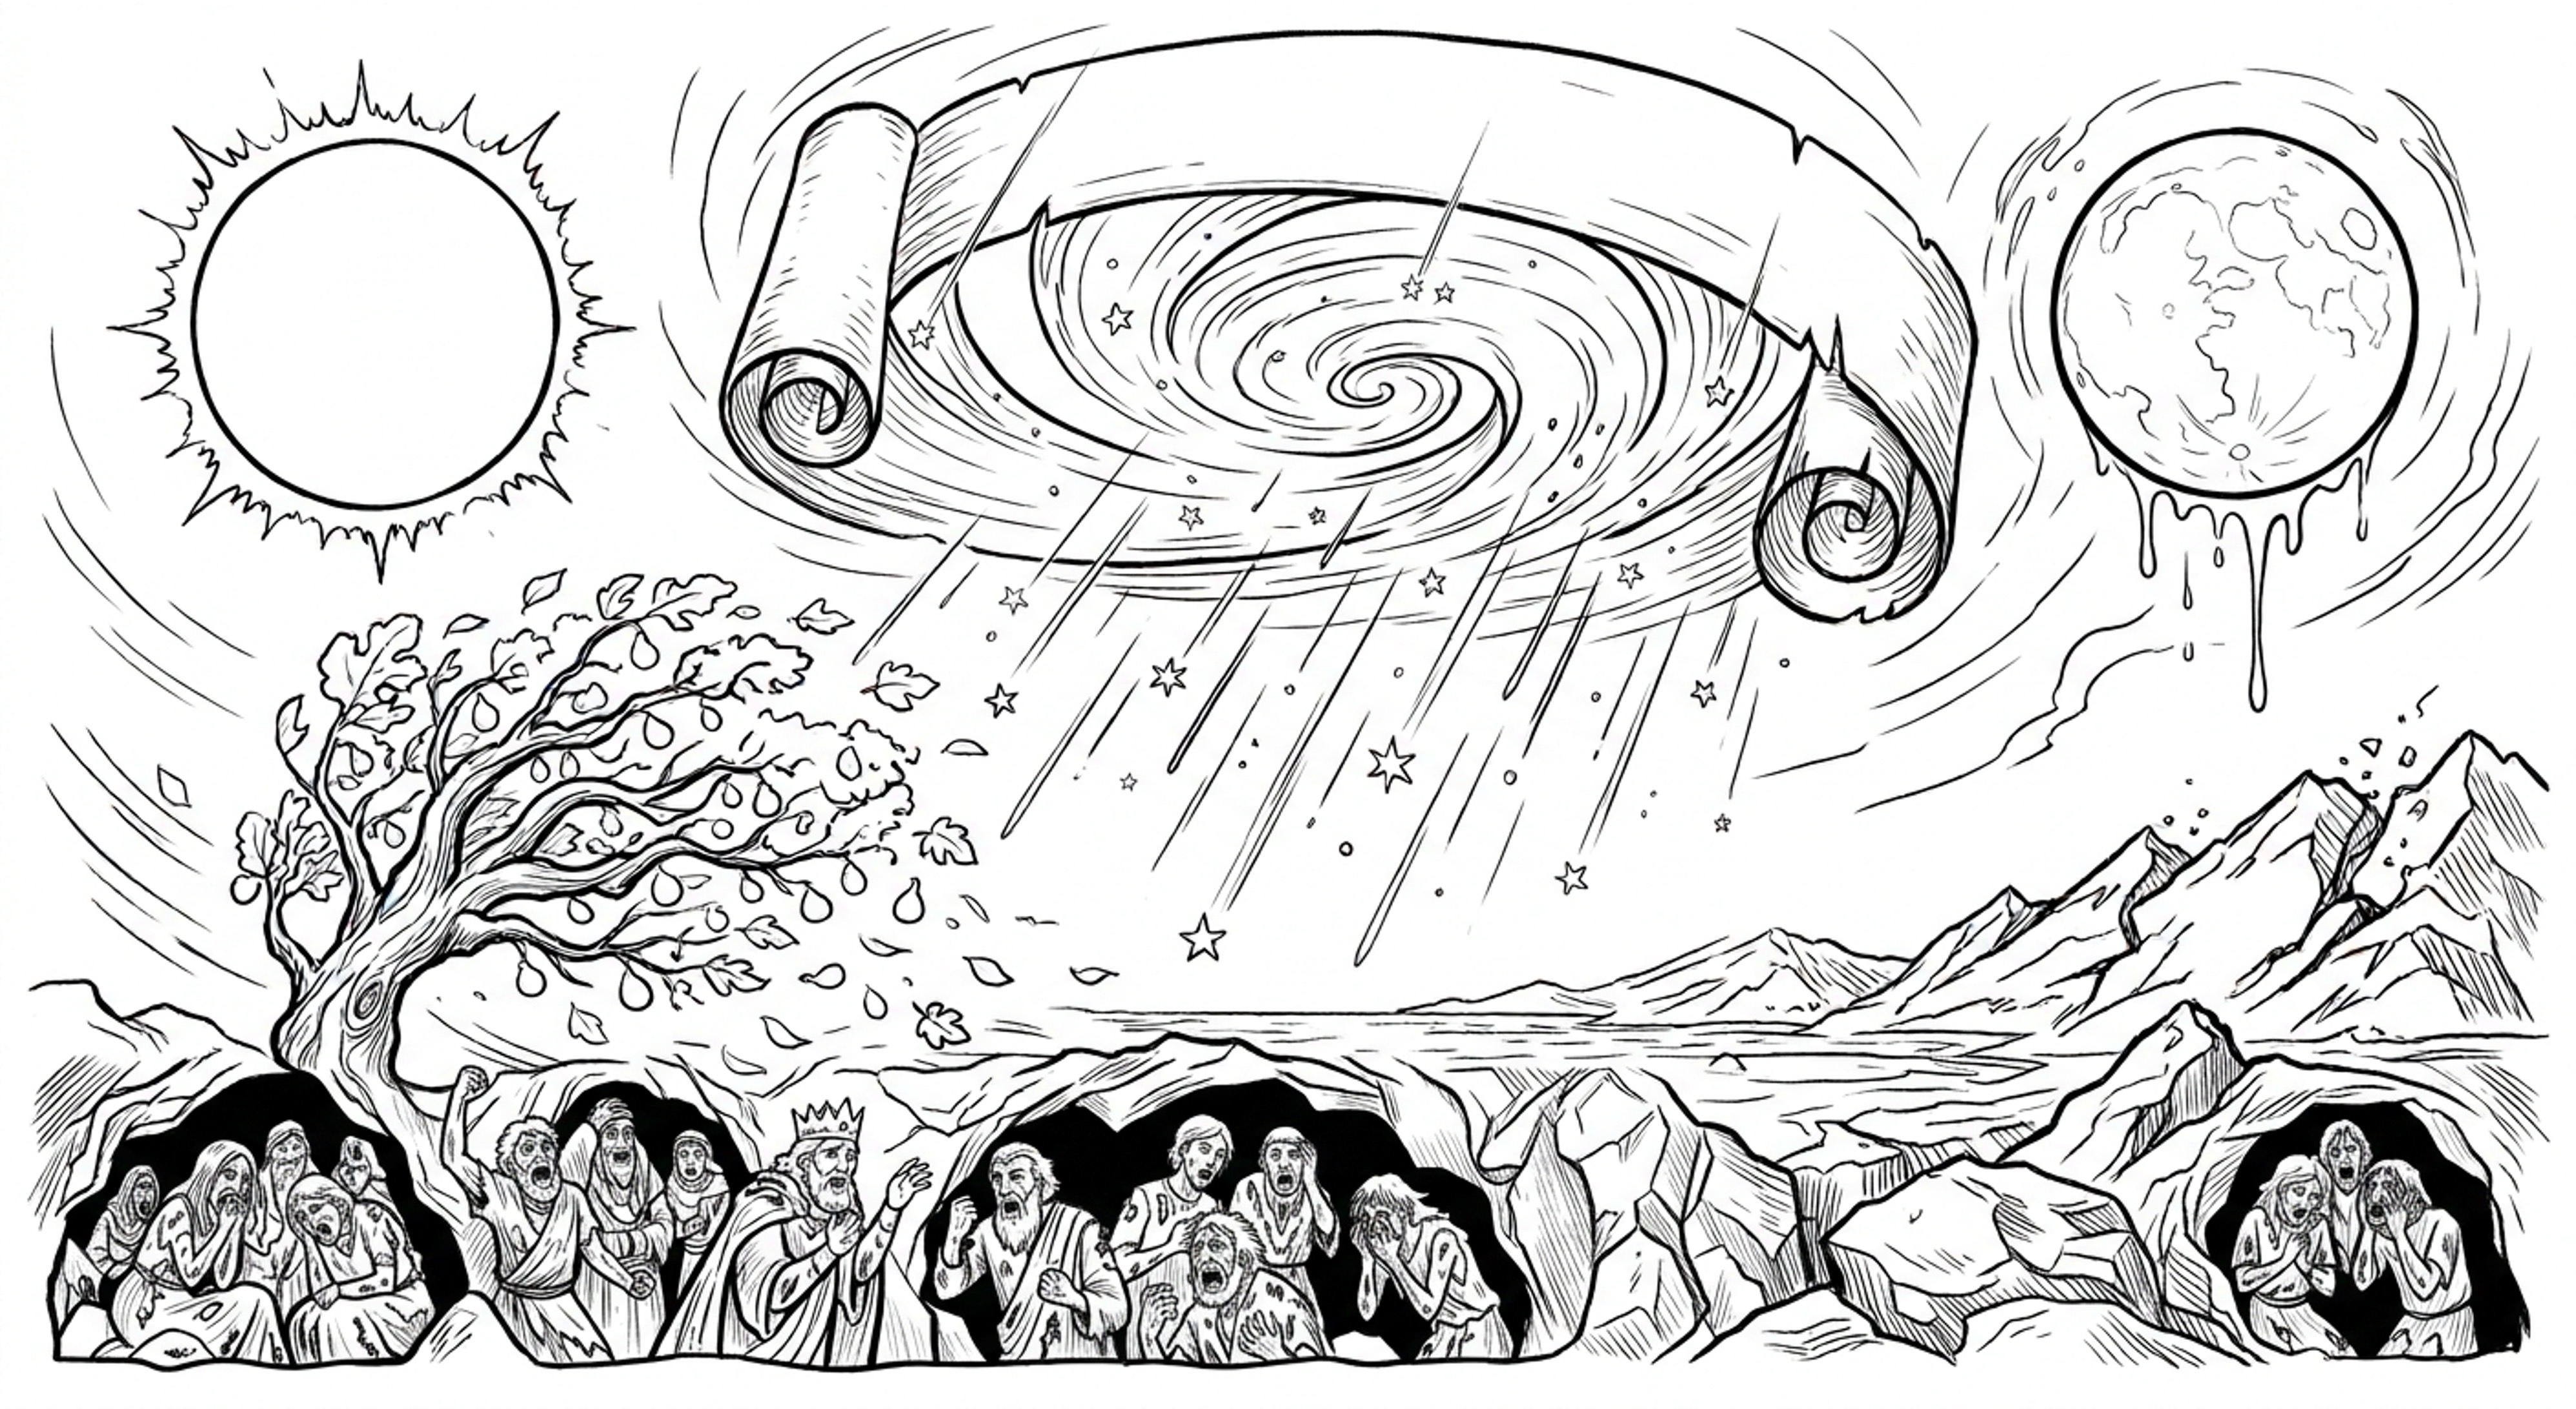
\includegraphics[
    width=1\textwidth,
    trim=0 0 0 0,
    clip]{images/seal_6th.jpg}
    \caption{The 6th Seal: The Stars Fall from the Sky}
    \label{fig:seal_6th}
\end{figure}

The heavens and the earth are shaken. The familiar order of creation seems to come apart, and the people of the earth find nowhere to hide. In terror, they ask who can stand before the righteous wrath of the Lamb.

Yet Revelation 7 will show us the answer. Those who have been redeemed by the blood of the Lamb will stand before the throne and before Him, as shown in Table \ref{tab:who-can-stand}.

{
\small
\renewcommand{\arraystretch}{1}
\begin{longtable}{p{0.43\textwidth} p{0.43\textwidth}}
\caption{Who can stand?}
\label{tab:who-can-stand} \\
\hline
Revelation 6:15--17 & Revelation 7:9--14 \\
\hline
\endfirsthead

\multicolumn{2}{l}{\small\itshape Table~\thetable\ (continued)} \\
\hline
Revelation 6:15--17 & Revelation 7:9--14 \\
\hline
\endhead

\hline
\endfoot

\hline
\endlastfoot

People hide from the face of God and the Lamb & A great multitude stands before God and the Lamb \\
They tremble at the coming day of wrath & They wear white robes and worship God \\
They ask, ``Who can stand?'' & The blood of the Lamb enables the redeemed to stand \\
\end{longtable}
}

This contrast captures the central message of these chapters.

When we face the righteous wrath of the Lamb, will we be able to stand before Him? The answer does not lie in our own good works or strength. It rests in the Lamb, who shed His blood for us, redeemed us, and cleansed us from sin.

Even today, Christ extends His gracious invitation to us. My hope is that every reader of this book will receive the Lamb's invitation rather than wait until that dreadful day and seek to hide from His presence.

If you have not yet turned to Christ, now is the time to repent and place your trust in His saving work. By the grace of the Lamb, you too may join the multitude clothed in white, standing before Him and giving glory and praise to God.

\subsection*{The First Six Seals and Matthew 24}

The Olivet Discourse, in which Jesus speaks about the events to come in Matthew 24, bears striking parallels to the first six seals in Revelation.
Table \ref{tab:seals-matthew24} shows the parallels.
{
\small
\renewcommand{\arraystretch}{1}
\begin{longtable}{>{\raggedright\arraybackslash}p{0.27\textwidth}
                  >{\raggedright\arraybackslash}p{0.33\textwidth}
                  >{\raggedright\arraybackslash}p{0.25\textwidth}}
\caption{The six seals of Revelation 6 and the signs in Matthew 24}
\label{tab:seals-matthew24} \\
\hline
Seal & Matthew 24 & Correspondence \\
\hline
\endfirsthead

\multicolumn{3}{l}{\small\itshape Table~\thetable\ (continued)} \\
\hline
Seal & Matthew 24 & Correspondence \\
\hline
\endhead

\endfoot

\endlastfoot

\ding{172} The white horse: its rider goes out conquering and to conquer &
\textsuperscript{4--5} Many come in Christ's name and deceive many &
False messiahs and deceptive claims of peace. \\
\hline
\ding{173} The red horse: peace is taken from the earth, and people kill one another &
\textsuperscript{6--7} Wars and rumors of wars; nation rises against nation and kingdom against kingdom &
War, violence, and social upheaval. \\
\hline
\ding{174} The black horse: scales and expensive grain &
\textsuperscript{7} Famines in various places &
Food shortages and economic hardship. \\
\hline
\ding{175} The pale horse: death and the realm of the dead &
\textsuperscript{7--9} Famines, earthquakes, and believers handed over to suffering &
Death, disasters, and affliction. \\
\hline
\ding{176} The martyrs cry out for justice &
\textsuperscript{9--13} Believers suffer persecution, are killed and hated, and are called to endure to the end &
Persecution, martyrdom, and perseverance. \\
\hline
\ding{177} Earthquake, darkened sun and moon, and falling stars &
\textsuperscript{29--30} The sun and moon are darkened, the stars fall, and the Son of Man appears in heaven &
Cosmic upheaval and the coming of the Son of Man. \\
\hline
\end{longtable}
}

Matthew 24 and the vision of the seven seals each have their own emphasis. Matthew stresses the need for Jesus' disciples to remain alert, endure to the end, and await the coming of the Son of Man. Revelation develops these themes through the vision of the Lamb opening the scroll, showing that history and judgment remain under the sovereign authority of Christ.

The parallels are significant, but they do not require every detail to correspond to an identical event or a precise timetable. Both passages call believers to discernment and endurance while keeping their eyes fixed on the Lord who will bring history to its appointed end.

\section{The Seventh Seal}

% Insert the licensed NIV text of Revelation 8:1 in the ScriptureBox below.

\begin{ScriptureBox}
\item[8:1] \textit{When he opened the seventh seal, there was silence in heaven for about half an hour.}
\end{ScriptureBox}

The seventh seal appears in Revelation 8:1. We introduce it here alongside the first six seals because it completes the sequence, even though the biblical account continues into the next chapter.

Unlike the first six seals, the seventh does not immediately portray a distinct calamity. Instead, it introduces the vision of the seven trumpets (8:2). Through these trumpets, God's judgments continue to unfold, carrying the vision into a new stage.

When the Lamb opens the seventh seal, silence falls over heaven for about half an hour. The silence is like a rest in a great symphony. The heavenly hosts fall still, and the entire court of heaven seems to hold its breath, awaiting the solemn and terrible movement that is about to begin.

This silence does not signal the end of judgment. It is a moment of awe-filled stillness before the next great movement of divine judgment breaks forth.

\subsection*{The Sequence of the Seven Seals, Seven Trumpets, and Seven Bowls}

The seventh seal introduces the seven trumpets. When the seventh trumpet sounds, a heavenly proclamation announces the kingdom of God and of Christ, and speaks of God's wrath, the judgment of the dead, and the rewarding of the prophets and saints (11:18).

Yet the seven bowls do not immediately follow the seventh trumpet. Between them stand the visions in Chapters 12--14: the woman and the dragon, the two beasts, the Lamb with the 144,000, and the messages of the three angels. In Chapter 15, John sees seven angels holding the seven last plagues, and is told that with them God's wrath is completed (15:1). Chapter 16 then describes the pouring out of the seven bowls.

To give readers an overview, Figure \ref{fig:seals_trumpets_bowls} illustrates the sequence of the seals, trumpets, and bowls. The following discussion addresses a related interpretive question.

\begin{figure}[htbp]
    \centering
    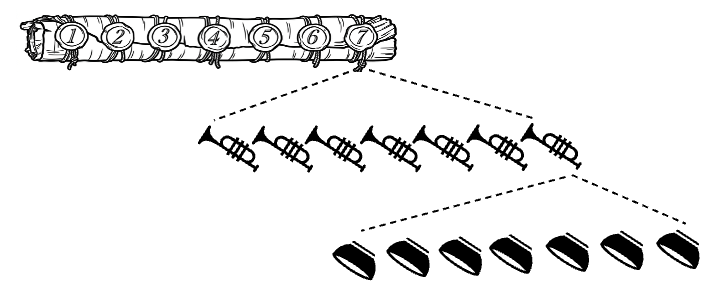
\includegraphics[
    width=1\textwidth,
    trim=0 0 0 0,
    clip]{images/seals_trumpets_bowls.png}
    \caption{The Sequence of the Seven Seals, Seven Trumpets, and Seven Bowls}
    \label{fig:seals_trumpets_bowls}
\end{figure}

Because many of the judgments among the seals, trumpets, and bowls appear to resemble one another, an important question naturally arises.

\subsection*{Do the Seven Seals, Seven Trumpets, and Seven Bowls Occur in Sequence, or Do They Recapitulate the Same Final Judgment?}

Read at face value, the seven seals, seven trumpets, and seven bowls appear in succession. But could they instead describe the same events from different perspectives, each time intensifying the portrayal of judgment? Interpreters have proposed two broad approaches to the relationship between these three series of visions. Table \ref{tab:seals-trumpets-bowls} shows the comparison.

{
\small
\renewcommand{\arraystretch}{1}
\begin{longtable}{>{\raggedright\arraybackslash}p{0.15\textwidth}|
                  >{\raggedright\arraybackslash}p{0.35\textwidth}|
                  >{\raggedright\arraybackslash}p{0.4\textwidth}}
\caption{Two views of the seals, trumpets, and bowls}
\label{tab:seals-trumpets-bowls} \\
\hline
 & Successive Judgments & Recapitulation with Increasing Intensity \\
\hline
\endfirsthead

\multicolumn{3}{l}{\small\itshape Table~\thetable\ (continued)} \\
\hline
 & Successive Judgments & Recapitulation with Increasing Intensity \\
\hline
\endhead

\endfoot

\endlastfoot

Seals & The seventh seal introduces the seven trumpets. & The seals portray God's judgment upon the world. \\
\hline
Trumpets & The trumpets follow the seventh seal. & The trumpets revisit the theme of judgment from another perspective and intensify it. \\
\hline
Bowls & The bowls follow the trumpets and bring God's wrath to its full expression. & The bowls present another recapitulation of divine judgment. \\
\hline
Evidence & The seventh seal introduces the trumpets, and the bowls appear after the trumpet visions. & The sixth seal, seventh trumpet, and seventh bowl all employ language associated with final judgment. \\
\hline
Strength & Emphasizes the apparent chronological sequence of the visions. & Helps explain the recurring images of cosmic upheaval, divine wrath, and judgment upon the nations. \\
\hline
\end{longtable}
}

These two approaches are not necessarily mutually exclusive in every respect. Interpreters who favor recapitulation do not always deny the sequence presented in the text. Rather, they understand that sequence as part of a literary structure in which related visions may overlap or portray events from different perspectives.

For this reason, we should be cautious about assigning each judgment to a specific modern historical event solely on the basis of the order in which the visions appear.

You may ask: When will the seven seals take place? Will they occur only during a future great tribulation, or did they begin in the apostolic age and continue until Christ's return? Could they also portray patterns of suffering and judgment that recur throughout history?

Christian theologians have offered several interpretations of these questions. I discuss them in greater detail in the appendix, ``Various Views of the End Times.''

We now turn to Revelation 7, where John sees 144,000 people sealed, followed by a multitude beyond counting, drawn from every nation, tribe, people, and language, standing before the throne and the Lamb.

\section{The Seal of the Living God Preserves His Servants}


\begin{ScriptureBox}

\item[7:1] After this I saw four angels standing at the four corners of the earth, holding back the four winds of the earth to prevent any wind from blowing on the land or on the sea or on any tree.

\item[7:2] Then I saw another angel coming up from the east, having the seal of the living God. He called out in a loud voice to the four angels who had been given power to harm the land and the sea:

\item[7:3] ``Do not harm the land or the sea or the trees until we put a seal on the foreheads of the servants of our God.''

\end{ScriptureBox}

You may have noticed that between the sixth and seventh seals, the narrative suddenly pauses to introduce Revelation 7 and the sealing of God's servants by the living God. Why is this vision placed here?

The answer lies in the question with which Revelation 6:17 ends: ``For the great day of their wrath has come, and who can withstand it?'' Revelation 7 responds directly. Those who belong to God—the servants who bear His seal and the multitude clothed in white—are seen standing before the throne and the Lamb.\footnote{Beale, G. K. (1999).}

The expression ``the four winds'' draws upon Old Testament imagery for forces that affect the whole earth.\footnote{Daniel 7:2 speaks of ``the four winds of heaven'' churning up the great sea; Jeremiah 49:36 describes God bringing the four winds against Elam and scattering its people in every direction.} We therefore need not evaluate ``the four corners of the earth'' or ``the four winds'' through the lens of modern geometry or meteorology. The point is not the physical shape of the earth, but God's authority over the whole world and His sovereign control over the timing of judgment.

Why are God's servants sealed before judgment proceeds? This is a central point of the vision. The seal is not an incidental detail added to the judgment scene; it identifies those who belong to God and expresses His redemptive care for them. Let us consider who receives this seal.

\section{The Twelve Tribes of Israel}

% Insert the licensed NIV text of Revelation 7:4 and 7:8 in the ScriptureBox below.

\begin{ScriptureBox}

\item[7:4] Then I heard the number of those who were sealed: 144,000 from all the tribes of Israel.

\item[7:5] From the tribe of Judah 12,000 were sealed,\\
from the tribe of Reuben 12,000,\\
from the tribe of Gad 12,000,

\item[7:6] from the tribe of Asher 12,000,\\
from the tribe of Naphtali 12,000,\\
from the tribe of Manasseh 12,000,

\item[7:7] from the tribe of Simeon 12,000,\\
from the tribe of Levi 12,000,\\
from the tribe of Issachar 12,000,

\item[7:8] from the tribe of Zebulun 12,000,\\
from the tribe of Joseph 12,000,\\
from the tribe of Benjamin 12,000.

\end{ScriptureBox}

John records that 144,000 people are sealed. Who are they? The number may be understood literally, though it may also carry symbolic significance. Three major interpretations are commonly proposed:

{
\small
\renewcommand{\arraystretch}{1}
\begin{longtable}{>{\raggedright\arraybackslash}p{2.4cm}
                  >{\raggedright\arraybackslash}p{6.6cm}}
\hline
Interpretation & Explanation \\
\hline
\endfirsthead

\hline
Interpretation & Explanation \\
\hline
\endhead

\endfoot

\endlastfoot

Israel &
The 144,000 are people sealed from the twelve tribes of Israel in the last days. \\
\hline
The church  &
The number represents the complete people of God, consisting of Jewish and Gentile believers. \\
\hline
Israel as a symbol &
The twelve tribes symbolize God's people in the last days, emphasizing His complete preservation of those who belong to Him. \\
\hline
\end{longtable}
}

Throughout Revelation, the number twelve appears repeatedly: the twelve tribes, the twelve apostles, the twelve gates, the twelve foundations, and the twelve gates of the New Jerusalem (Revelation 21:12--14). The carefully structured number 144,000 therefore resonates with Revelation's recurring use of twelve to represent the fullness and completeness of God's people.

Some writers attempt to identify precisely which individuals belong to this number. Such speculation, however, seems to go beyond what this passage is intended to establish. The central emphasis is that God knows those who belong to Him. When judgment comes upon the earth, He does not forget His people; He recognizes them and holds them within His sovereign care.

\section{The Worship of All Nations and the Salvation of the Lamb}


\begin{ScriptureBox}

\item[7:9] After this I looked, and there before me was a great multitude that no one could count, from every nation, tribe, people and language, standing before the throne and before the Lamb. They were wearing white robes and were holding palm branches in their hands.

\item[7:10] And they cried out in a loud voice:\\
\hspace*{1em}``Salvation belongs to our God,\\
\hspace*{2em}who sits on the throne,\\
\hspace*{1em}and to the Lamb.''

\item[7:11] All the angels were standing around the throne and around the elders and the four living creatures. They fell down on their faces before the throne and worshiped God,

\item[7:12] saying:\\
\hspace*{1em}``Amen!\\
\hspace*{1em}Praise and glory\\
\hspace*{2em}and wisdom and thanks and honor\\
\hspace*{2em}and power and strength\\
\hspace*{1em}be to our God for ever and ever.\\
\hspace*{1em}Amen!''

\end{ScriptureBox}

What a magnificent sight! A multitude beyond counting gathers in joyful, ordered worship. People from every nation, tribe, people, and language stand together before the throne and the Lamb. Here is a unity that human power could never create: a redeemed people brought together by the salvation of God.

Have you received this salvation? Are you confident that one day you will be among that vast multitude, standing before the throne and joining their song of praise?

If you have not yet received the salvation of Jesus Christ, today is an opportunity to pause, consider His invitation, and turn to Him. Jesus Christ gave His life for sinners and rose from the dead. He calls you to repent, trust in Him, and receive the grace He freely offers.

Will you receive His grace today?

\section{From Great Tribulation to Eternal Rest}

% Insert the licensed NIV text of Revelation 7:13--17 in the ScriptureBox below.

\begin{ScriptureBox}

\item[7:13] Then one of the elders asked me, ``These in white robes---who are they, and where did they come from?''

\item[7:14] I answered, ``Sir, you know.''\\
And he said, ``These are they who have come out of the great tribulation; they have washed their robes and made them white in the blood of the Lamb.

\item[7:15] Therefore,\\
\hspace*{1em}``they are before the throne of God\\
\hspace*{2em}and serve him day and night in his temple;\\
\hspace*{1em}and he who sits on the throne\\
\hspace*{2em}will shelter them with his presence.

\item[7:16] \hspace*{1em}`Never again will they hunger;\\
\hspace*{2em}never again will they thirst.\\
\hspace*{1em}The sun will not beat down on them,'\\
\hspace*{2em}nor any scorching heat.

\item[7:17] \hspace*{1em}For the Lamb at the center of the throne\\
\hspace*{2em}will be their shepherd;\\
\hspace*{1em}`he will lead them to springs of living water.'\\
\hspace*{2em}`And God will wipe away every tear from their eyes.'\,''
% NIV footnotes for 7:16--17 (omitted; add as \footnote if wanted):
%   7:16 ``beat down on them'' --- Isaiah 49:10
%   7:17 ``springs of living water'' --- Isaiah 49:10
%   7:17 ``every tear from their eyes'' --- Isaiah 25:8
% CHECK NIV: footnote references quoted from memory; verify against Bible Gateway.

\end{ScriptureBox}

Blood ordinarily stains garments red. Yet here we are told that the blood of the Lamb makes the robes of the redeemed white. The image recalls Isaiah 1:18, where God promises that sins as scarlet will become white as snow, and sins as crimson will become like wool.

The victory described here is not the triumph of believers who have escaped tribulation through their own strength. It is the victory of the Lamb, whose blood accomplishes redemption and brings God's people into His eternal presence.

From the deliverance of the Exodus, through the prophets' promises of restoration, to the sacrifice of the Lamb and the new creation, the whole story of redemption points toward one ultimate hope: God Himself will be the God of His people; the Lamb Himself will be their Shepherd; and God will wipe away every tear from their eyes.\footnote{Wu Rongchu, ``Revelation, Episode 12: Sealed on the Forehead and Kept from Harm,'' Grace Baptist Church, Taipei, September 1, 2021, \texttt{https://www.gbc.org.tw/2021/09/20210902/}.}

Notice the wonder contained in this promise. The Lamb who was slain becomes the Shepherd who leads His people. The One whose blood was shed to redeem them now guides them to springs of living water. Those who once knew hunger, thirst, suffering, and grief will no longer be abandoned to these sorrows. Their final destination is not merely survival beyond judgment, but life in the presence of God.

This is the hope that sustains the church through suffering. The present world is not the final word. Persecution does not erase God's promises; death does not undo the Lamb's victory; and tears will not flow forever. The Shepherd who gave His life for His sheep will bring them safely home.

\section*{Discussion Questions}

\begin{enumerate}

\item When we encounter injustice, how can we follow the example of the martyrs under the fifth seal? How can we seek justice while entrusting judgment to God rather than taking revenge into our own hands?

\item Why are the people of the earth terrified when the sixth seal is opened? What does their question, ``Who can withstand it?'' teach us about our need for the salvation of Christ?

\item The blood of the Lamb makes the robes of the redeemed white. How does this image deepen our understanding of Christ's saving work, and how should this truth shape our daily lives?

\end{enumerate}
